\documentclass[11pt,a4paper,titlepage]{report}
\usepackage[utf8]{inputenc}
\usepackage{amsmath}
\usepackage{amsfonts}
\usepackage{amssymb}
\usepackage{makeidx}
\usepackage{graphicx}
\begin{document}
	\title{Hasil Simulasi}
	\maketitle
	
	\section*{Simulasi ke-I}
	\subsection*{Tabel}
	\begin{tabular}{|c|c|}
		\hline Generasi & Fitness \\ 
		\hline 0 & 0.93 \\ 
		\hline 1 & 0.92 \\ 
		\hline 2 & 0.92 \\ 
		\hline 3 & 0.91 \\ 
		\hline 4 & 0.91 \\ 
		\hline 5 & 0.89 \\ 
		\hline 6 & 0.89 \\ 
		\hline 7 & 0.93 \\ 
		\hline 8 & 0.93 \\ 
		\hline 9 & 0.93 \\ 
		\hline 10 & 0.89 \\
		\hline
	\end{tabular} 
	\subsection*{Individu Terbaik}
	\begin{description}
		\item[Koordinat AP] [4, 11], [8, 48], [10, 76], [11, 61], [14,79], [15, 5], [17, 33], [19, 13], [20, 71], [21, 60], [25, 34]
		\item[Fitness] 0.9275
	\end{description}
	\newpage
	\subsection*{Gambar}
	\begin{figure*}[h]
	\centering
	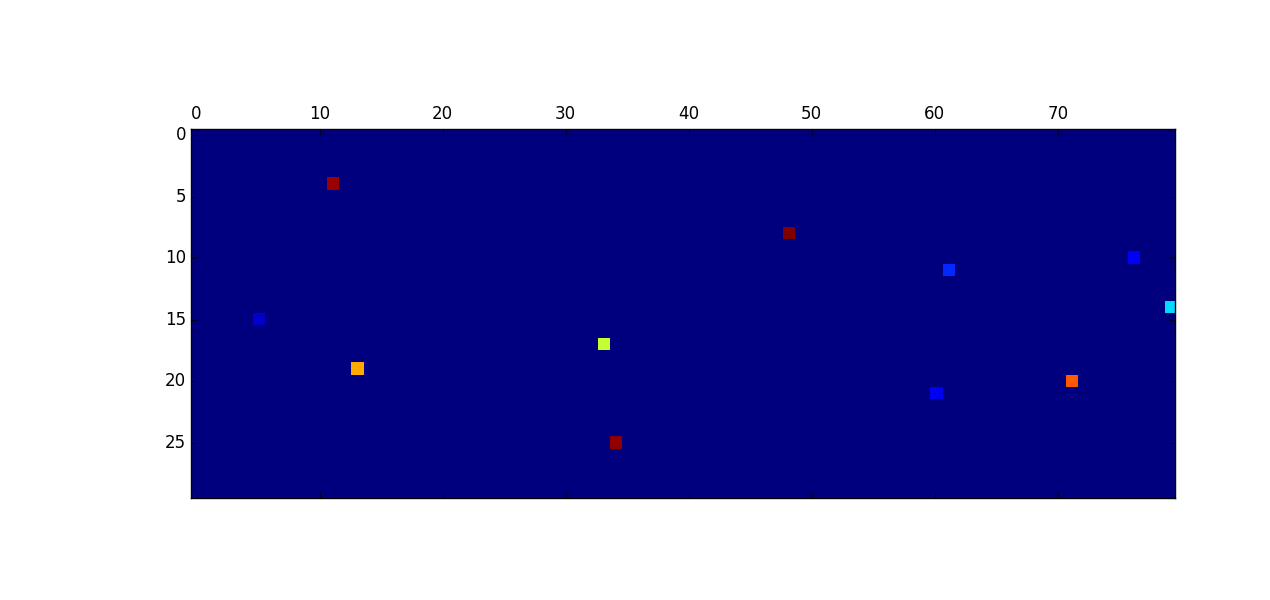
\includegraphics[width=0.9\linewidth]{apLoc_01}
	\caption{Koordinat AP}
	\label{fig:apLoc_01}
	\end{figure*}
	\begin{figure}[h]
	\centering
	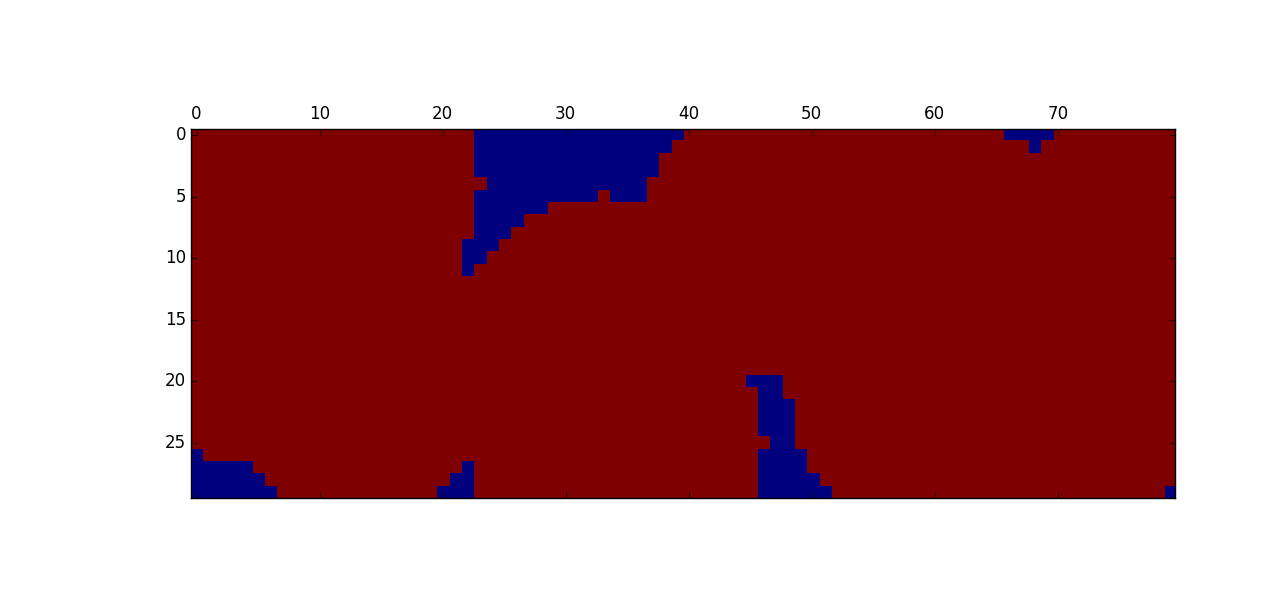
\includegraphics[width=0.9\linewidth]{coverage_01}
	\caption{Covarage Area}
	\label{fig:coverage_01}
	\end{figure}
	\newpage
	\section*{Simulasi ke-II}
	\subsection*{Tabel}
	\begin{tabular}{|c|c|}
		\hline Generasi & Fitness \\ 
		\hline 0 & 0.98 \\ 
		\hline 1 & 0.90 \\ 
		\hline 2 & 0.90 \\ 
		\hline 3 & 0.88 \\ 
		\hline 4 & 0.91 \\ 
		\hline 5 & 0.91 \\ 
		\hline 6 & 0.95 \\ 
		\hline 7 & 0.95 \\ 
		\hline 8 & 0.92 \\ 
		\hline 9 & 0.92 \\ 
		\hline 10 & 0.95 \\
		\hline
	\end{tabular} 
	\subsection*{Individu Terbaik}
	\begin{description}
		\item[Koordinat AP] [5, 63], [7, 77], [9, 21], [9, 45], [11, 5], [15, 64], [17, 48], [25, 6], [25, 28], [26, 73], [28, 61]
		\item[Fitness] 0.9754
	\end{description}
	\newpage
	\subsection*{Gambar}
	\begin{figure*}[h]
		\centering
		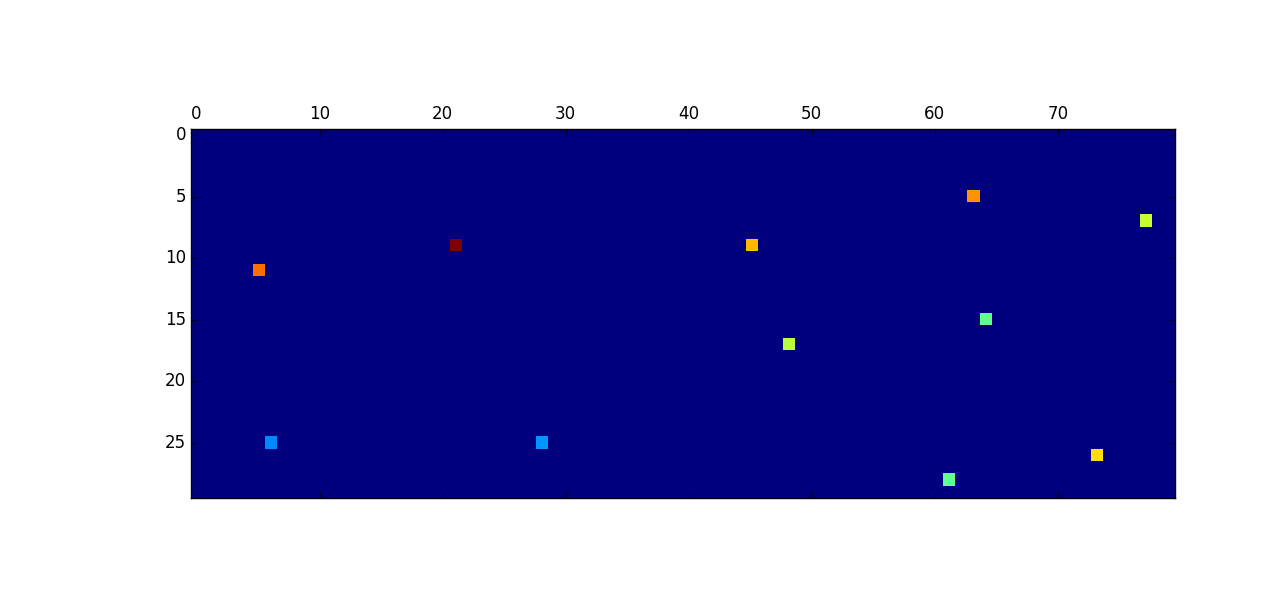
\includegraphics[width=0.9\linewidth]{apLoc_02}
		\caption{Koordinat AP}
		\label{fig:apLoc_02}
	\end{figure*}
	\begin{figure}[h]
		\centering
		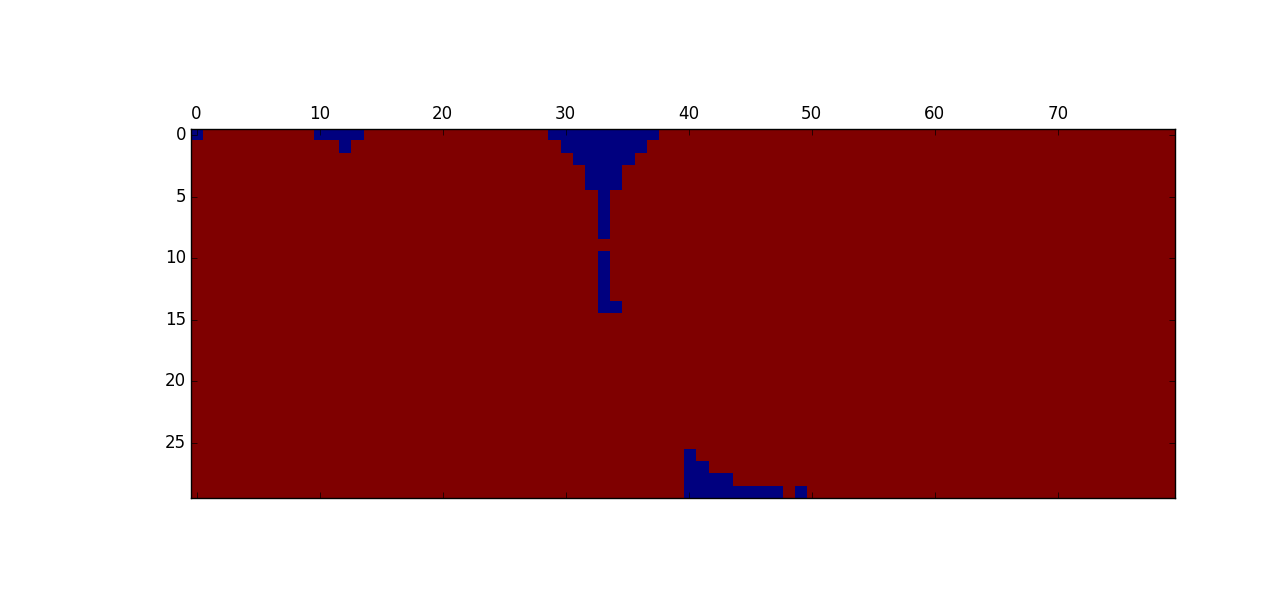
\includegraphics[width=0.9\linewidth]{coverage_02}
		\caption{Covarage Area}
		\label{fig:coverage_02}
	\end{figure}
	\newpage
	\section*{Simulasi ke-III}
	\subsection*{Tabel}
	\begin{tabular}{|c|c|}
		\hline Generasi & Fitness \\ 
		\hline 0 & 0.92 \\ 
		\hline 1 & 0.92 \\ 
		\hline 2 & 0.92 \\ 
		\hline 3 & 0.92 \\ 
		\hline 4 & 0.90 \\ 
		\hline 5 & 0.90 \\ 
		\hline 6 & 0.90 \\ 
		\hline 7 & 0.89 \\ 
		\hline 8 & 0.92 \\ 
		\hline 9 & 0.92 \\ 
		\hline 10 & 0.92 \\
		\hline
	\end{tabular} 
	\subsection*{Individu Terbaik}
	\begin{description}
		\item[Koordinat AP] [22, 15], [21, 43], [8, 65], [9, 66], [21, 52], [18, 59], [5, 22], [21, 9], [7, 0], [6, 43], [28, 67]
		\item[Fitness] 0.9246
	\end{description}
	\newpage
	\subsection*{Gambar}
	\begin{figure*}[h]
		\centering
		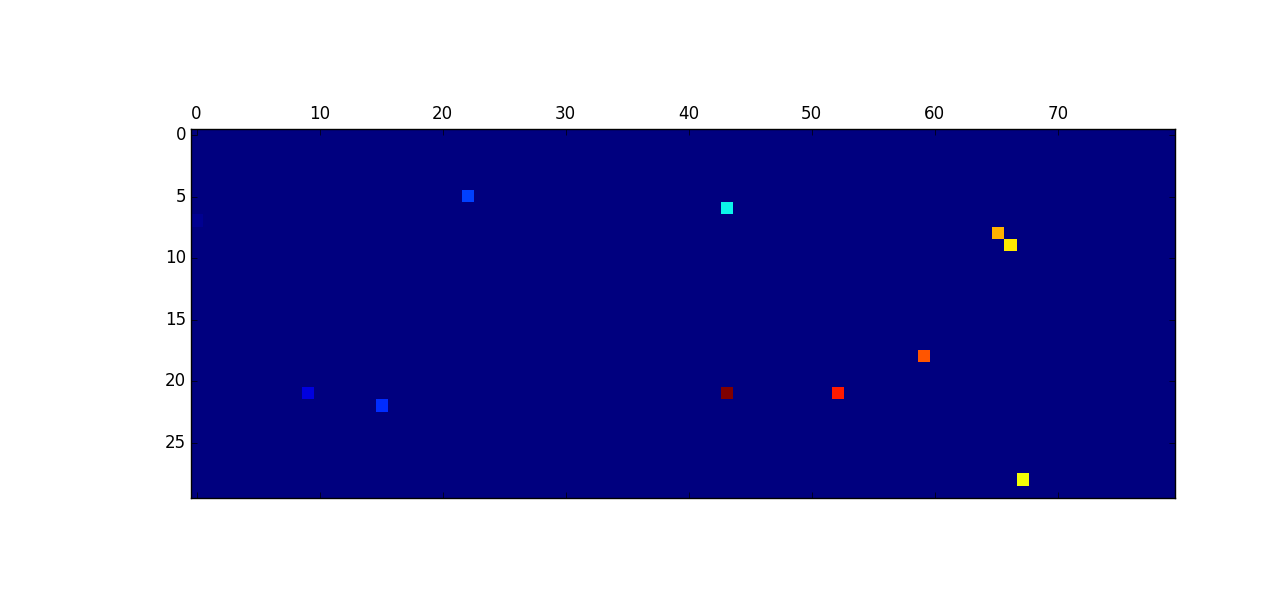
\includegraphics[width=0.9\linewidth]{apLoc_03}
		\caption{Koordinat AP}
		\label{fig:apLoc_03}
	\end{figure*}
	\begin{figure}[h]
		\centering
		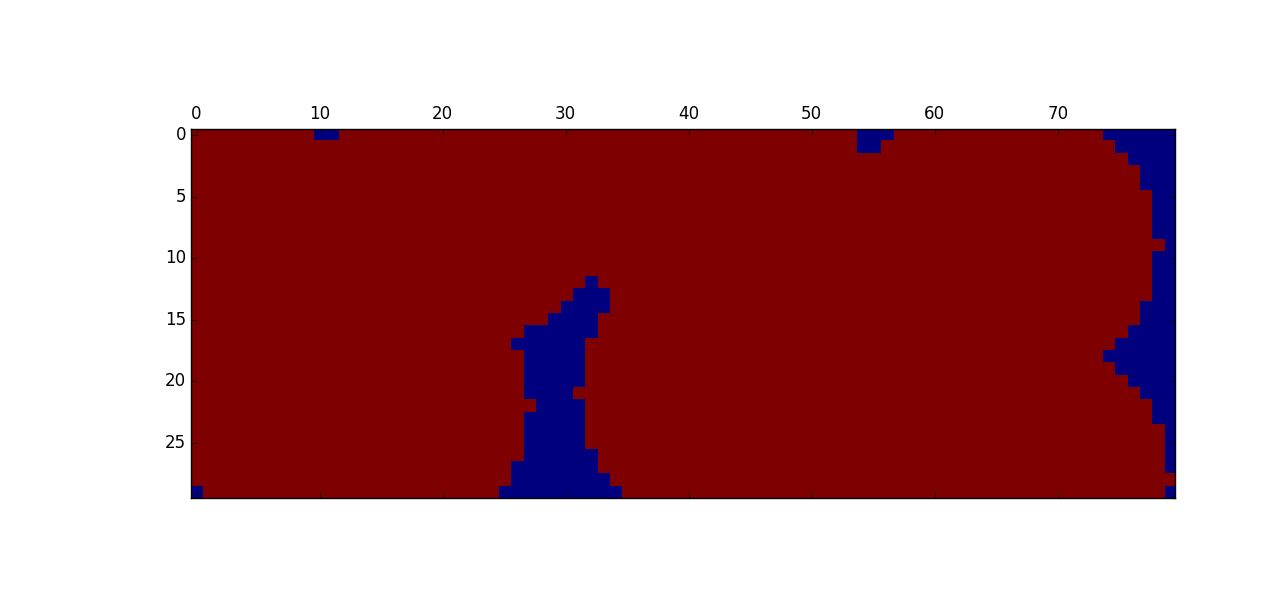
\includegraphics[width=0.9\linewidth]{coverage_03}
		\caption{Covarage Area}
		\label{fig:coverage_03}
	\end{figure}
	\newpage
	\section*{Simulasi ke-IV}
	\subsection*{Tabel}
	\begin{tabular}{|c|c|}
		\hline Generasi & Fitness \\ 
		\hline 0 & 0.91 \\ 
		\hline 1 & 0.91 \\ 
		\hline 2 & 0.90 \\ 
		\hline 3 & 0.88 \\ 
		\hline 4 & 0.88 \\ 
		\hline 5 & 0.88 \\ 
		\hline 6 & 0.88 \\ 
		\hline 7 & 0.89 \\ 
		\hline 8 & 0.89 \\ 
		\hline 9 & 0.89 \\ 
		\hline 10 & 0.89 \\
		\hline
	\end{tabular} 
	\subsection*{Individu Terbaik}
	\begin{description}
		\item[Koordinat AP] [1, 21], [8, 63], [10, 35], [13, 23], [13, 55], [21, 24], [18, 8], [21, 74], [26, 6], [27, 46], [29, 9]
		\item[Fitness] 0.9129
	\end{description}
	\newpage
	\subsection*{Gambar}
	\begin{figure*}[h]
		\centering
		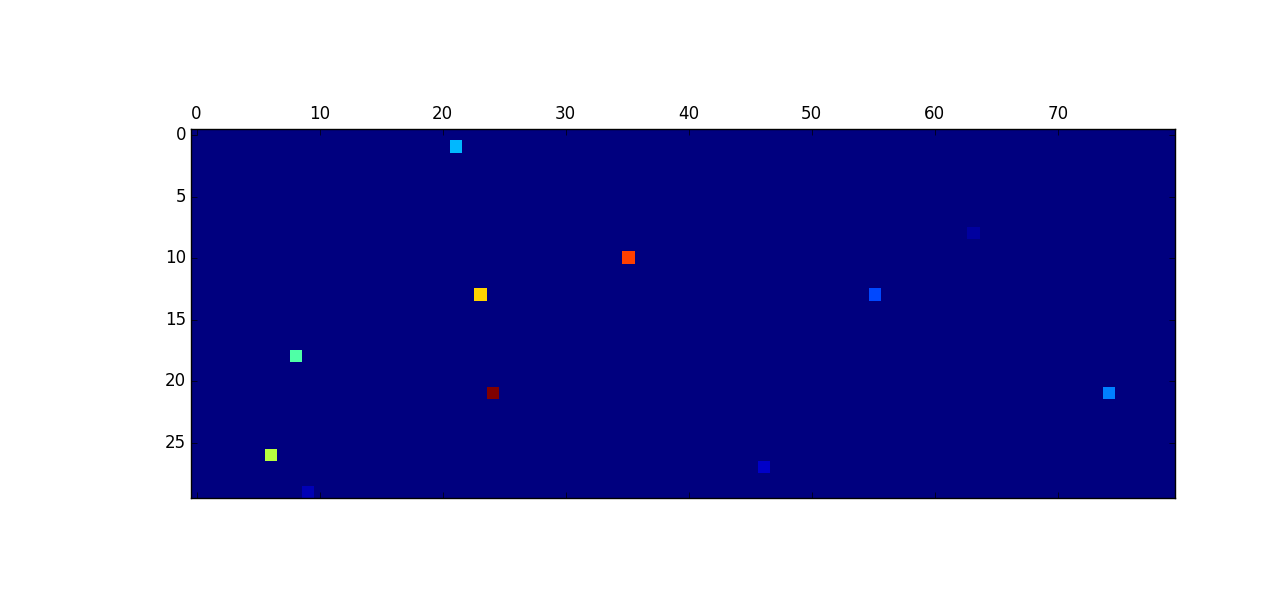
\includegraphics[width=0.9\linewidth]{apLoc_04}
		\caption{Koordinat AP}
		\label{fig:apLoc_04}
	\end{figure*}
	\begin{figure}[h]
		\centering
		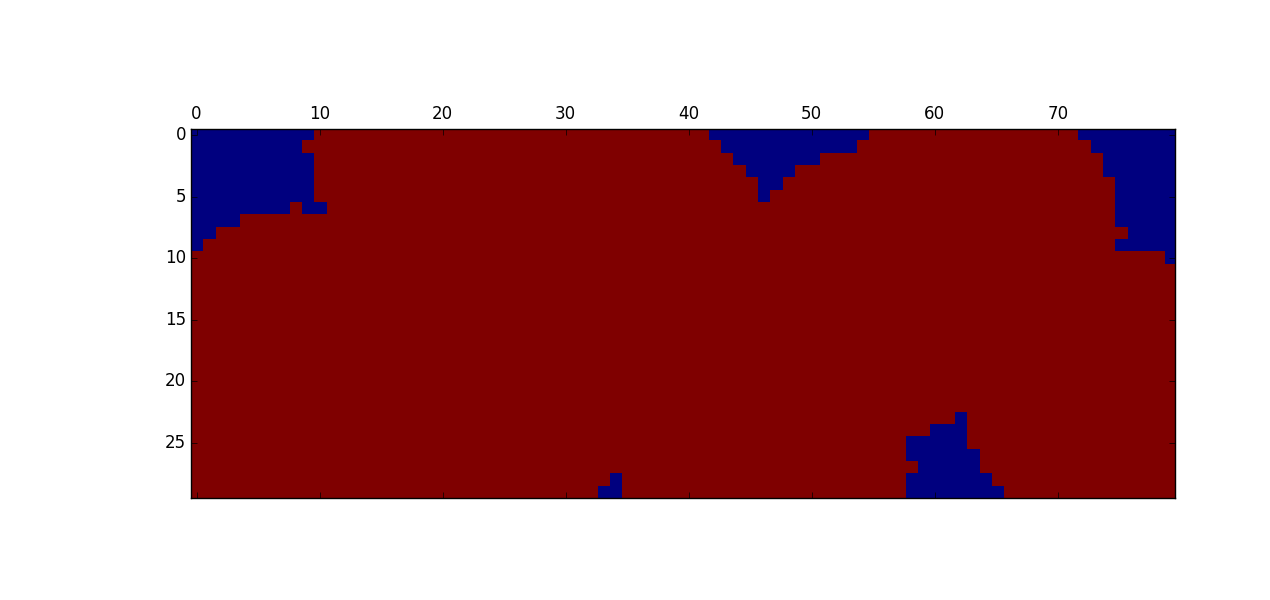
\includegraphics[width=0.9\linewidth]{coverage_04}
		\caption{Covarage Area}
		\label{fig:coverage_04}
	\end{figure}
	\newpage
	\section*{Simulasi ke-V}
	\subsection*{Tabel}
	\begin{tabular}{|c|c|}
		\hline Generasi & Fitness \\ 
		\hline 0 & 0.90 \\ 
		\hline 1 & 0.89 \\ 
		\hline 2 & 0.89 \\ 
		\hline 3 & 0.88 \\ 
		\hline 4 & 0.87 \\ 
		\hline 5 & 0.87 \\ 
		\hline 6 & 0.90 \\ 
		\hline 7 & 0.90 \\ 
		\hline 8 & 0.88 \\ 
		\hline 9 & 0.88 \\ 
		\hline 10 & 0.88 \\
		\hline
	\end{tabular} 
	\subsection*{Individu Terbaik}
	\begin{description}
		\item[Koordinat AP] [1, 54], [2, 9], [2, 14], [17, 41], [10, 27], [11, 3], [12, 71], [13, 41], [13, 12], [23, 52], [28, 13]
		\item[Fitness] 0.9033
	\end{description}
	\newpage
	\subsection*{Gambar}
	\begin{figure*}[h]
		\centering
		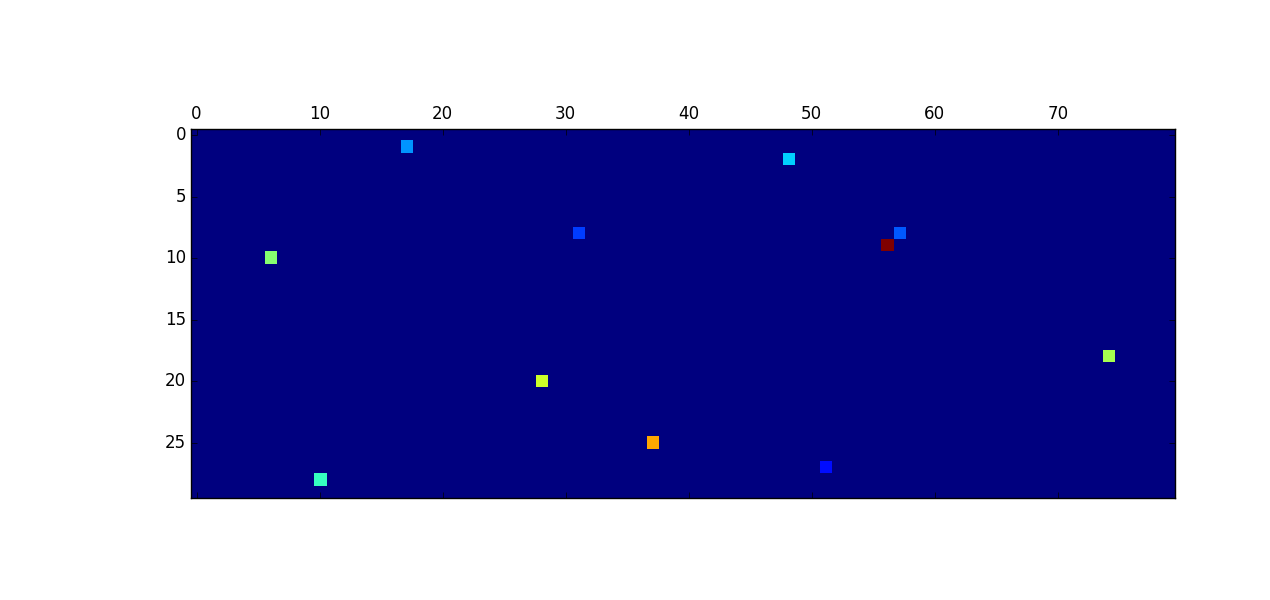
\includegraphics[width=0.9\linewidth]{apLoc_05}
		\caption{Koordinat AP}
		\label{fig:apLoc_05}
	\end{figure*}
	\begin{figure}[h]
		\centering
		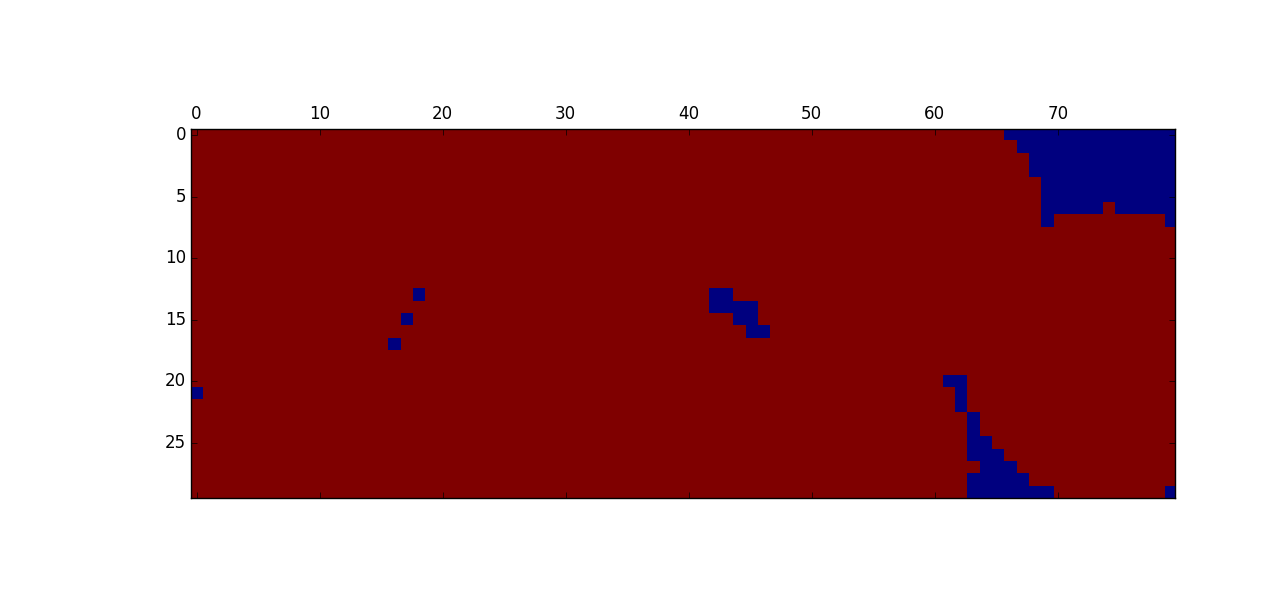
\includegraphics[width=0.9\linewidth]{coverage_05}
		\caption{Covarage Area}
		\label{fig:coverage_05}
	\end{figure}
\end{document}